\chapter{Equational Theorem Proving}
Mathematics, particularly the field of mathematical theorem proving, is intrinsically linked to the notion of intelligence. \textcolor{blue}{Automatic theorem proving} represents a significant branch of artificial intelligence dedicated to the application of AI techniques within mathematics. The domain of \emph{automatic theorem proving} is extensive enough to warrant several volumes. However, due to time constraints, this chapter will focus exclusively on \textcolor{blue}{equational theorem proving}. In \emph{equational theorem proving}, we start with a collection of axioms, which are expressed as equations, and seek to determine which additional equations can be inferred from these axioms. As an illustration, consider a \textcolor{blue}{group} $\mathcal{G}$, defined as a quadruple:
\\[0.2cm]
\hspace*{1.3cm}
$\mathcal{G} = \langle G, e, \circ, i \rangle$
\\[0.2cm]
subject to the following conditions:
\begin{itemize}
    \item $G$ is a set, whose elements are referred to as \textcolor{blue}{group elements}.
    \item $e \in G$, signifying that $e$ is an element of $G$. This element, $e$, is known as the
          \textcolor{blue}{left-neutral element} due to reasons that will be clarified subsequently. 
    \item $\circ: G \times G \rightarrow G$, indicating that $\circ$ is a binary operation on $G$ that maps
          pairs of group elements to a group element. This operation is termed the \textcolor{blue}{multiplication}
          of the group $\mathcal{G}$. 
    \item $i: G \rightarrow G$, denoting that $i$ is a unary operation on $G$ mapping each group element to
          another group element. For any element $x \in G$, the result $i(x)$ is known as the
          \textcolor{blue}{left-inverse} of $x$. 
    \item The set $G$, along with the operations defined, must satisfy the \textcolor{blue}{group axioms}:  
      \begin{enumerate}[(a)]
          \item $e \circ x = x$ for all $x \in G$,
          \item $i(x) \circ x = e$ for all $x \in G$,
          \item $(x \circ y) \circ z = x \circ (y \circ z)$ for all $x, y, z \in G$.
      \end{enumerate}
\end{itemize}
In \href{https://en.wikipedia.org/wiki/Abstract_algebra}{abstract algebra}, it is shown that these axioms imply
the equation 
\\[0.2cm]
\hspace*{1.3cm}
$x \circ i(x) = e$, \quad i.e.~the left inverse of any group element $x$ is also a right inverse of $x$.
\\[0.2cm]
A possible proof runs as follows:
$$
\begin{array}{lcll}
  x \circ i(x) & = & e \circ \bigl(x \circ i(x)\bigr) & \mbox{because $e$ is left-neutral} \\
               & = & \Bigl(i\bigl(x \circ i(x)\bigr) \circ \bigl(x \circ i(x)\bigr)\Bigr) \circ \bigl(x \circ i(x)\bigr)
                   & \mbox{because $i\bigl(x \circ i(x)\bigr) \circ \bigl(x \circ i(x)\bigr) = e$} \\
               & = & i\bigl(x \circ i(x)\bigr) \circ \Bigl(\bigl(x \circ i(x)\bigr) \circ \bigl(x \circ i(x)\bigr)\Bigr)
                   &  \mbox{associativity} \\
               & = & i\bigl(x \circ i(x)\bigr) \circ \biggl(x \circ \Bigl(i(x) \circ \bigl(x \circ i(x)\bigr)\Bigr)\biggr) 
                   &  \mbox{associativity} \\
               & = & i\bigl(x \circ i(x)\bigr) \circ \biggl(x \circ \Bigl(\bigl(i(x) \circ x\bigr) \circ i(x)\Bigr)\biggr) 
                   &  \mbox{associativity} \\
               & = & i\bigl(x \circ i(x)\bigr) \circ \Bigl(x \circ \bigl(e \circ i(x)\bigr)\Bigr) 
                   &  \mbox{because $i(x) \circ x = e$} \\
               & = & i\bigl(x \circ i(x)\bigr) \circ \bigl(x \circ i(x)\bigr) 
                   &  \mbox{because $e \circ i(x) = i(x)$} \\
               & = & e 
                   & \mbox{because $i(z) \circ z = e$ where $z = x \circ i(x)$.}
\end{array}
$$

The formulation of proofs for such equations is far from straightforward. However, a systematic method exists
for addressing these and related equational challenges. In this chapter, we introduce an algorithm capable of
autonomously generating equational proofs similar to those discussed earlier. This algorithm is recognized as
the \href{https://en.wikipedia.org/wiki/Knuth-Bendix_completion_algorithm}{Knuth-Bendix completion algorithm},
a significant contribution by Donald E. Knuth and Peter B. Bendix \cite{knuth:1970}. 

The structure of this chapter is organized as follows:
\begin{enumerate}
\item Initially, we will formally define \textcolor{blue}{equational proofs} and \textcolor{blue}{term
      rewriting}, setting the foundation for subsequent discussions. 
\item Subsequently, we explore abstract properties of relations, introducing essential concepts such as
      \textcolor{blue}{confluence} and providing proofs for the \textcolor{blue}{Church-Rosser theorem} and
      \textcolor{blue}{Newman's lemma}. 
\item The third section delves into term orderings, including the introduction of the
      \textcolor{blue}{Knuth-Bendix ordering}, which plays a pivotal role in the algorithm's process. 
\item The final section is dedicated to a detailed presentation of the \textcolor{blue}{Knuth-Bendix completion
      algorithm}, illustrating its application and significance in automatic theorem proving. 
\end{enumerate}

\section{Equational Proofs}
This section defines the notion of an \blue{equational proof} precisely and discusses how equational proofs can
be carried out via \blue{term rewriting}.  In order to do this, we have to define a number of more elementary
notions like \blue{functions symbols}, \blue{variables}, \blue{terms}, and \blue{substitutions}.  We begin with 
the notion of a signature.

\begin{Definition}[Signature]
  A \blue{signature} \index{signature} is a triple of the form
  \\[0.2cm]
  \hspace*{1.3cm} $\Sigma = \langle \mathcal{V}, \mathcal{F}, \textsl{arity} \rangle$,
  \\[0.2cm]
  where we have the following: 
  \begin{enumerate}
  \item $\mathcal{V}$ is the set of \blue{variables}. \index{variable}
  \item $\mathcal{F}$ is the set of \blue{function symbols}. \index{function symbol}
  \item $\textsl{arity}$ is a function such that
        \\[0.2cm]
        \hspace*{1.3cm}
        $\textsl{arity}: \mathcal{F} \rightarrow \mathbb{N}$.
        \\[0.2cm]
        If we have $\textsl{arity}(f) = n$, then $f$ is said to be an \blue{$n$-ary function symbol}.
  \item We have $\mathcal{V} \cap \mathcal{F} = \{\}$, i.e.~variables are different from function symbols. \eoxs
  \end{enumerate}
\end{Definition}

\example
The signature of \blue{group theory} $\Sigma_G$ can be defined as follows:
\begin{enumerate}[(a)]
\item $\mathcal{V} := \{ w, x, y, z \}$,
\item $\mathcal{F} := \{ e, i, \circ \}$,
\item $\textsl{arity} := \{ e \mapsto 0, i \mapsto 1, \circ \mapsto 2 \}$,
  
      i.e.~$e$ is a constant symbol, $i$ is a unary function symbol, and $\circ$ is a binary function symbol.
\item $\Sigma = \langle \mathcal{V}, \mathcal{F}, \textsl{arity} \rangle$. \eoxs
\end{enumerate}

\noindent
Having defined the notion of a signature we proceed to define terms.

\begin{Definition}[Term,  $\mathcal{T}_\Sigma$]
  If $\Sigma = \langle \mathcal{V}, \mathcal{F}, \textsl{arity} \rangle$ is a signature, the set of
  \blue{$\Sigma$-terms} \index{term} \index{$\Sigma$-term} \blue{$\mathcal{T}_\Sigma$}
  \index{$\mathcal{T}_\Sigma$} is defined inductively:
  \begin{enumerate}
  \item For every variable $x \in \mathcal{V}$ we have $x \in \mathcal{T}_\Sigma$.
  \item If $f \in \mathcal{F}$ and $\textsl{arity}(f) = 0$, then $f \in \mathcal{T}_\Sigma$.
  \item If $f \in \mathcal{F}$ and $n := \textsl{arity}(f) > 0$ and, furthermore, $t_1,\cdots,t_n \el \mathcal{T}_\Sigma$,  then we have
        \\[0.2cm]
        \hspace*{1.3cm} $f(t_1,\cdots,t_n) \el \mathcal{T}_\Sigma$.
        \eoxs
  \end{enumerate}
\end{Definition}

\example
Given the signature $\Sigma_G$ defined above, we have the following:
\begin{enumerate}
\item $x \in \mathcal{T}_{\Sigma_G}$,
  
      because every variable is a $\Sigma_{G}$-term.
\item $e \in \mathcal{T}_{\Sigma_G}$.
\item $\circ(e,x) \in \mathcal{T}_{\Sigma_G}$.
\item $\circ\bigl(\circ(x,y),z\bigr) \in \mathcal{T}_{\Sigma_G}$.
\end{enumerate}

\remark
Later on we will often use an \blue{infix notation} for binary function symbols.  In general, if $f$ is a
binary function symbol, then the term $f(t_1,t_2)$ is written as $t_1 \,f\; t_2$.  If this notation would
result in an ambiguity because either $t_1$ or $t_2$ is also written in infix notation, then we use parenthesis
to resolve the ambiguity.  For example, we will write
\\[0.2cm]
\hspace*{1.3cm}
$(x \circ y) \circ z$ \quad instead of \quad $\circ\bigl(\circ(x,y),z\bigr) \in \mathcal{T}_{\Sigma_G}$.  
\\[0.2cm]
Note that we cannot write the term $\circ\bigl(\circ(x,y),z\bigr)$ as $x \circ y \circ z$ because that notation
is ambiguous, since it can be interpreted as either $(x \circ y) \circ z$ or $x \circ (y \circ z)$.
\eoxs

\begin{Definition}[$\Sigma$-Equation]
  Assume a signature $\Sigma$ is given.  A \blue{$\Sigma$-equation}\index{$\Sigma$-equation} is a pair $\pair(s,t)$ such
  that both $s$ and $t$ are $\Sigma$-terms.  The $\Sigma$-equation $\pair(s,t)$ is written as
  \\[0.2cm]
  \hspace*{1.3cm}
  $s \approx t$.  \eoxs
\end{Definition}

\remark
We use the notation $s \approx t$ instead of the notation $s=t$ in order to distinguish between the notion of a
$\Sigma$-\blue{equation} and the notion of \blue{equality} of terms.  So when $s$ and $t$ are $\Sigma$-terms and we
write $s = t$ we do mean that $s$ and $t$ are literally the same terms, while writing $s \approx t$
means that we are interested in the logical consequences that would follow from the assumption that the
interpretation of $s$ and $t$ are the same in certain \blue{$\Sigma$-algebras}.  The notion of a $\Sigma$-algebra
is defined next.  \eoxs

\begin{Definition}[$\Sigma$-Algebra]
  Assume a signature $\Sigma = \langle \mathcal{V}, \mathcal{F}, \textsl{arity} \rangle$ is given.  A
  \blue{$\Sigma$-algebra}\footnote{
    The notion of a $\Sigma$-algebra is a notion that is used both in logic and in
    \href{https://en.wikipedia.org/wiki/Universal_algebra}{universal algebra}.  In universal algebra, a
    $\Sigma$-algebra is also known as an \blue{algebraic structure}.  This notion is not related to and should
    not be confused with the notion of a \blue{$\sigma$-algebra}, which is a notion used in the field of
    \href{https://en.wikipedia.org/wiki/Measure_(mathematics)}{measure theory}.  Note that the notion used in
    measure theory is always written with a lower case $\sigma$, while the notion used in logic is written with
    a capital $\Sigma$. 
  } is a pair of the form $\textfrak{A} = \pair(A, \mathcal{J})$ where:
  \begin{enumerate}
  \item $A$ is a nonempty set that is called the \blue{universe} of the $\Sigma$-algebra $\textfrak{A}$.
  \item $\mathcal{J}$ is the \blue{interpretation} of the function symbols.  Technically, $\mathcal{J}$ is a
        function that is defined on the set $\mathcal{F}$ of all function symbols.  For every function symbol
        $f \in \mathcal{F}$ we have that 
        \\[0.2cm]
        \hspace*{1.3cm}
        $\mathcal{J}(f): A^{\textsl{arity}(f)} \rightarrow A$, 
        \\[0.2cm]
        i.e. $\mathcal{J}(f)$ is a function from $A^n$ to $A$ where $n$ is the arity of the function symbol
        $f$.

        If $\textfrak{A} = \pair(A, \mathcal{J})$ is a $\Sigma$-algebra, then the function $\mathcal{J}(f)$ is 
        usually written more concisely as $f^\textfrak{A}$. 
  \end{enumerate}
  The set of all $\Sigma$-algebras is written as $\mathtt{Alg}(\Sigma)$. \eoxs
\end{Definition}

\example
In this example we construct a $\Sigma_G$-algebra where $\Sigma_G$ is the signature of group theory defined
earlier.  We define $G := \{ 0, 1 \}$ and define the interpretations $\mathcal{J}(f)$ for $f \in \{e, i, \circ
\}$ as follows:
\begin{enumerate}
\item $\mathcal{J}(e) := 0$.
\item $\mathcal{J}(i) := \bigl\{ 0 \mapsto 0, 1 \mapsto 1 \bigr\}$.
\item $\mathcal{J}(\circ) := \bigl\{ \pair(0,0) \mapsto 0,
                                    \pair(0,1) \mapsto 1,
                                    \pair(1,0) \mapsto 1,
                                    \pair(1,1) \mapsto 0
                            \bigr\}$.
\end{enumerate}
Then $\textfrak{G} = \pair(G, \mathcal{J})$ is a $\Sigma_G$-algebra.  \eoxs

\remark
Alternatively, we could have given the interpretation of the multiplication symbol $\circ$ as
\\[0.2cm]
\hspace*{1.3cm}
$\mathcal{J}(\circ)(x, y) := (x + y) \;\texttt{\%}\; 2$.

\begin{Definition}[Variable Assignment] \hspace*{\fill} \linebreak
  If $\Sigma = \langle \mathcal{V}, \mathcal{F}, \textsl{arity} \rangle$ is a signature and $\textfrak{A} = \pair(A, \mathcal{J})$ is a $\Sigma$-algebra, then a
  \blue{variable assignment}\index{variable assignment} is a function of the form
  \\[0.2cm]
  \hspace*{1.3cm}
  $I: \mathcal{V}  \rightarrow A$
  \\[0.2cm]
  that is the variable assignment $I$ maps every variable $v \in \mathcal{V}$ to a value in the set $A$.
  
\end{Definition}

\begin{Definition}[Evaluation, Valid Equation] \hspace*{\fill} \linebreak
  If $\Sigma = \langle \mathcal{V}, \mathcal{F}, \textsl{arity} \rangle$ is a signature,
  $\textfrak{A} = \pair(A, \mathcal{J})$ is a $\Sigma$-algebra, and $I$ is a \blue{variable assignment}\index{variable assignment}, 
  then we can \blue{evaluate} $\Sigma$-terms in $\textfrak{A}$ as follows:
  \begin{enumerate}
  \item $\texttt{eval}(x, I) := I(x)$ \quad for all $x \in \mathcal{V}$.
  \item $\texttt{eval}(c, I) := c^\textfrak{A}$ \quad for every constant symbol $c \in \mathcal{F}$.
  \item $\texttt{eval}\bigl(f(t_1,\cdots,t_n), I\bigr) := f^\textfrak{A}\bigl(\texttt{eval}(t_1,I),\cdots,\texttt{eval}(t_n,I)\bigr)$.
  \end{enumerate}
  A $\Sigma$-equation $s \approx t$ is \blue{valid} in the $\Sigma$-algebra $\textfrak{A}$ iff we have
  \\[0.2cm]
  \hspace*{1.3cm}
  $\texttt{eval}(s,I) = \texttt{eval}(t,I)$ for all variable assignments $I:\mathcal{V} \rightarrow A$.
  \\[0.2cm]
  This is written as
  \\[0.2cm]
  \hspace*{1.3cm}
  $\textfrak{A} \models s \approx t$
  \\[0.2cm]
  and we say that $\textfrak{A}$ \blue{satisfies} the equation $s \approx t$.
  \eoxs
\end{Definition}

\example
Continuing the previous example we have the following:
\begin{enumerate}
\item $\textfrak{G} \models e \circ x \approx x$,
\item $\textfrak{G} \models i(x) \circ x \approx e$,
\item $\textfrak{G} \models (x \circ y) \circ z \approx x \circ (y \circ z)$. \eoxs
\end{enumerate}

\begin{Definition}[$E$-Variety]
  Assume that $\Sigma$ is a signature and $E$ is a set of $\Sigma$-equations.  The collection of all
  $\Sigma$-structures that satisfy every equation from $E$ is called the \blue{$E$-variety}\index{$E$-variety}.
  \\[0.2cm]
  \hspace*{1.3cm}
  $\texttt{Variety}(E) := \bigl\{ \textfrak{A}\in \mathtt{Alg}(\Sigma) \bigm| 
                             \forall (s \approx t) \in E: \textfrak{A} \models s \approx t \bigr\}$.
  \\[0.2cm]
  To put it differently, the $\Sigma$-structure $\textfrak{A}$ is a member of $\mathtt{Variety}(E)$ iff
  \\[0.2cm]
  \hspace*{1.3cm}
  $\textfrak{A} \models s \approx t$ \quad for every equation $s \approx t$ in $E$. \eoxs
\end{Definition}

\example
Define $E := \bigl\{ e \circ x = x, i(x) \circ x = e, (x \circ y) \circ z = x \circ (y \circ z) \bigr\}$.
This set of equations defines the variety of \blue{groups}.  You can check that the $\Sigma_G$-algebra
$\textfrak{G}$ is a member of this variety and hence it is a group.  
\eoxs

Given a set of $\Sigma$-equations $E$ it is natural to ask which other equations are \blue{logical consequences} of
the equations in $E$.  This notion is defined below. 

\begin{Definition}[Logical Consequence]
  Assume a signature $\Sigma$ and a set $E$ of $\Sigma$-equations to be given.
  Then the equation $s \approx t$ is a \blue{logical consequence} of $E$ iff we have
  \\[0.2cm]
  \hspace*{1.3cm}
  $\textfrak{A} \models s \approx t$ \quad for every $\textfrak{A} \in \mathtt{Variety}(E)$.
  \\[0.2cm]
  If $s \approx t$ is a logical consequence of the set of equations $E$, then this is written as
  \\[0.2cm]
  \hspace*{1.3cm}
  $E \models s \approx t$.
  \\[0.2cm]
  Therefore we have $E \models s \approx t$ if and only if every $\Sigma$-algebra that satisfies all equations
  from $E$ also satisfies the equation $s \approx t$. \eoxs
\end{Definition}

\example
In the introduction of this chapter we have already seen that if we define
$E := \bigl\{ e \circ x = x, i(x) \circ x = e, (x \circ y) \circ z = x \circ (y \circ z) \bigr\}$,
then we have
\\[0.2cm]
\hspace*{1.3cm}
$E \models x \circ i(x) \approx e$.  \eox

The notion $E \models s \approx t$ is a \blue{semantic notion}.  We cannot hope to implement this notion directly
because if a set of equations $E$ and a possible logical consequence $s \approx t$ is given, there are, in
general, infinitely many $\Sigma$-algebras that have to be checked.  Fortunately, the notion 
$E \models s \approx t$ has a \blue{syntactical analog} $E \vdash s \approx t$ (read: $E$ proves $s \approx t$)
that can be implemented and that is at least \blue{semi-decidable}, i.e.~we can create a program that given 
a set of equations $E$ and an equation $s \approx t$ will return \texttt{True} if $E \vdash s \approx t$ holds, and will
either return \texttt{False} or run forever if $E \vdash s \approx t$ does not hold.  Even more fortunately,
\href{https://en.wikipedia.org/wiki/G%C3%B6del%27s_completeness_theorem}{G\"{o}dels completeness theorem} 
implies that the syntactical notion coincides with the semantic notion, i.e.~we have
\\[0.2cm]
\hspace*{1.3cm}
$E \models s \approx t$ \quad if and only if \quad $E \vdash s \approx t$.

\subsection{A Calculus for Equality}
In this subsection we assume a signature $\Sigma$ and a set of $\Sigma$-equations $E$ to be given.  
Our goal is to define the provability notion $E \vdash s \approx t$, which is read as \blue{$E$ proves $s \approx t$}.
However, in order to do this we first need to define 
the notion of a \blue{substitution}.

\begin{Definition}[$\Sigma$-Substitution]
  Assume that a signature $\Sigma = \langle \mathcal{V}, \mathcal{F}, \textsl{arity} \rangle$ is given.
  A \blue{$\Sigma$-substitution} $\sigma$ is a map of the form
  \\[0.2cm]
  \hspace*{1.3cm}
  $\sigma: \mathcal{V} \rightarrow \mathcal{T}_\Sigma$ 
  \\[0.2cm]
  such that the set $\textsl{dom}(\sigma) := \bigl\{ x \in \mathcal{V} \mid \sigma(x) \not= x \bigr\}$ is finite.
  If we have $\textsl{dom}(\sigma) = \{ x_1, \cdots, x_n \}$ and $t_i = \sigma(x_i)$ for all $i = 1, \cdots, n$,
  then we use the following notation:
  \\[0.2cm]
  \hspace*{1.3cm}
  $\sigma = \{ x_1 \mapsto t_1, \cdots, x_n \mapsto t_n \}$.
  \\[0.2cm]
  The set of all $\Sigma$-Substitutions is denoted as $\mathtt{Subst}(\Sigma)$.
  \eoxs
\end{Definition}

A substitution $\sigma = \{ x_1 \mapsto t_1, \cdots, x_n \mapsto t_n \}$ can be \blue{applied} to a term $t$
by replacing the variables $x_i$ with the terms $t_i$.  We will use the postfix notation \blue{$t\sigma$} to denote the
\blue{application} of the substitution $\sigma$ to the term $t$.  Formally, the notation $t \sigma$ is defined
by induction on $t$:
\begin{enumerate}
\item $x \sigma := \sigma(x)$ \quad for all $x \in \mathcal{V}$.
\item $c \sigma = c$ \quad for every constant $c \in \mathcal{F}$.
\item $f(t_1, \cdots, t_n) \sigma := f\bigl(t_1\sigma, \cdots, t_n\sigma\bigr)$.
\end{enumerate}

\begin{Definition}[$E \vdash s \approx t$] \hspace*{\fill} \linebreak
  Given a signature $\Sigma$ and a set of $\Sigma$-equations $E$, the notion
  $E \vdash s \approx t$ is defined inductively.
  \begin{enumerate}
  \item $E \vdash s \approx t$ \quad for every $\Sigma$-equations $(s \approx t) \in E$. \hspace*{\fill} (\blue{Axioms})
  \item $E \vdash s \approx s$ \quad for every $\Sigma$-term $s$. \hspace*{\fill} (\blue{Reflexivity})
  \item If $E \vdash s \approx t$, then $E \vdash t \approx s$.  \hspace*{\fill} (\blue{Symmetry})
  \item If $E \vdash r \approx s$ and $E \vdash s \approx t$, then $E \vdash r \approx t$.  
        \hspace*{\fill} (\blue{Transitivity})
  \item If $\textsl{arity}(f) = n$ and $E \vdash s_i \approx t_i$ for all $i \in \{1,\cdots,n\}$, \\
        then $E \vdash f(s_1,\cdots,s_n) \approx f(t_1,\cdots,t_n)$.
        \hspace*{\fill} (\blue{Congruence})
  \item If $E \vdash s \approx t$ and $\sigma$ is a $\Sigma$-substitution, then $E \vdash s\sigma \approx
  t\sigma$. 
        \hspace*{\fill} (\blue{Stability})
  \end{enumerate}
  We read $E \vdash s \approx t$ as \blue{\mbox{$E$ proves $s \approx t$}}.
  \eoxs
\end{Definition}
The definition of $E \vdash s \approx t$ given above is due to 
\href{https://en.wikipedia.org/wiki/Gottfried_Wilhelm_Leibniz}{Gottfried Wilhelm}
\href{https://leibniz.com/en/keks-original}{Leibniz}.

\subsection{Equational Proofs}
It turns out that, although it is possible to implement the notion $E \vdash \approx t$ directly, it is much
more efficient to refine this notion a little bit.  To this end we need to introduce the notion of a
\blue{position} $u$ in a term $t$, the notion of the \blue{subterm} of a given term $t$ at a given position,
and the notion of \blue{replacing} a subterm at a given position by another term.  We define these notions
next. 

\begin{Definition}[Positions of a Term $t$, $\Pos(t)$] \hspace*{\fill} \\
  Given a term $t$ the set of all \blue{positions} of $t$ is written as $\Pos(t)$ and is defined by
  induction on $t$:
  \begin{enumerate}
  \item $\Pos(x) := \bigl\{ [\;] \bigr\}$ \quad for every variable $x$.
  \item $\Pos(c) := \bigl\{ [\;] \bigr\}$ \quad for every constant $c$.
  \item $\Pos\bigl(f(t_1,\cdots,t_n)\bigr) := 
         \bigl\{ [\;] \bigr\} \cup \bigcup\limits_{i=1}^n \bigl\{ [i] + u \mid u \in \Pos(t_i) \bigr\}$ 
        \quad for every term $f(t_1,\cdots,t_n)$. \eoxs
  \end{enumerate}
\end{Definition}

\begin{Definition}[Subterm at a given Position, $t/u$] \hspace*{\fill} \\
  Given a term $t$ and a position $u \in \Pos(t)$, the \blue{subterm of $t$ at position $u$} is
  written as $t/u$.  This expression is defined by induction on $u$.
  \begin{enumerate}
  \item $t/[\;] := t$,
  \item $f(t_1,\cdots,t_n)/\bigl([i]+u\bigr) := t_i/u$.  \eoxs
  \end{enumerate}
\end{Definition}

\begin{Definition}[Subterm Replacement, \mbox{$t[u \mapsto s]$}] \hspace*{\fill} \\
  Given a term $t$, a position $u \in \Pos(t)$, and a term $s$, the expression
  $t[u \mapsto s]$ denotes the term that results from $t$ when the subterm $t/u$ is replaced by the term 
  $s$.  This expression is defined by induction on $u$.
  \begin{enumerate}
  \item $t\bigl[ [\;] \mapsto s \bigr] := s$,
  \item $f(t_1,\cdots,t_n)\bigl[ [i]+u \mapsto s \bigr] := f(t_1, \cdots, t_{i-1},t_i[u \mapsto s], t_{i+1},\cdots, t_n)$.  
        \eoxs
  \end{enumerate}
\end{Definition}
  
\example
Define $t := (x \circ y) \circ z$.  Then we have
\\[0.2cm]
\hspace*{1.3cm}
$\Pos\bigl((x \circ y) \circ z\bigr) = \bigl\{ [\;], [1], [1,1], [1,2], [2]\bigr\}$.
\\[0.2cm]
Furthermore, we have the following:
\begin{enumerate}

\item $\bigl((x \circ y) \circ z\bigr)/[\;] = (x \circ y) \circ z$,
\item $\bigl((x \circ y) \circ z\bigr)/[1] = x \circ y$, and
\item $\bigl((x \circ y) \circ z\bigr)/[1,2] = y$.
\end{enumerate}
We also have
\\[0.2cm]
\hspace*{1.3cm}
$\bigl((x \circ y) \circ z\bigr)\bigl[[1] \mapsto y \circ x\bigr] = (y \circ x) \circ z$. \eox

\begin{Definition}[$\leftrightarrow_E$]
  Given a set of $\Sigma$-equations $E$ and two $\Sigma$-terms $s$ and $t$ we define that
  \\[0.2cm]
  \hspace*{1.3cm}
  $s \leftrightarrow_E t$
  \\[0.2cm]
  holds if and only if the following conditions are satisfied:
  \begin{enumerate}[(a)]
  \item There exists an equation $l \approx r$  such that either $(l \approx r) \in E$ or $(r \approx l) \in  E$.
  \item There is a position $u \in \Pos(s)$ and a substitution $\sigma$ such that $s/u = l\sigma$.
  \item $t = s[u \mapsto r\sigma]$. \eox
  \end{enumerate}
\end{Definition}
To put this is words: We have $s \leftrightarrow_E t$ iff there is an equation $l \approx r$ such that
either the equation $l \approx r$ or the equation $r \approx l$ is an element of the set of equations $E$ and,
furthermore, $s$ contains the subterm $l\sigma$ and $t$ results from $s$ by replacing the subterm $l\sigma$
with the subterm $r\sigma$. 

\example
If we have $E = \bigl\{ i(x) \circ x \approx e \bigr\}$ then
\\[0.2cm]
\hspace*{1.3cm}
$\bigl(i(a) \circ a\bigr) \circ b \;\leftrightarrow_E\; e \circ b$
\\[0.2cm]
because the right hand side $e \circ b$ results from the left hand side $\bigl(i(a) \circ a\bigr) \circ b$ by
replacing the subterm $i(a) \circ a$ that occurs at position $[1]$ by the term $e$.
This is possible because the equation $i(x) \circ x \approx e$ tells us that $i(a) \circ a$ is equal to $e$.
\eod

Next, we define the relation $\leftrightarrow_E^*$ as the \blue{reflexive and transitive closure} of the relation
$\leftrightarrow_E$.
\begin{Definition}[$\leftrightarrow_E^*$]
  For $\Sigma$-terms $s$ and $t$ the notion $s \leftrightarrow_E^* t$ is defined inductively as follows:
  \begin{enumerate}
  \item We have $s \leftrightarrow_E^* s$ for every $\Sigma$-term $s$.
  \item If $s \leftrightarrow_E t$, then $s \leftrightarrow_E^* t$.
  \item If $u$ is a $\Sigma$-term such that both $s \leftrightarrow_E u$ and $u \leftrightarrow_E^* t$ holds,
        then we have $s \leftrightarrow_E^* t$. \eod
  \end{enumerate}
\end{Definition}

\noindent
Given this definition it is now possible to show the following theorem.

\begin{Theorem}
  If $E$ is a set of equations and $s \approx t$ is an equation, then we have
  \\[0.2cm]
  \hspace*{1.3cm}
  $E \vdash s \approx t$ \quad if and only if \quad $s \leftrightarrow_E^* t$.
\end{Theorem}
For each of the two directions that has to be proven, the proof can be done by a straightforward, but tedious
induction. 

\subsection{Proofs via Rewriting}
The implementation of the relation $\leftrightarrow_E$ remains inefficient due to the dual utility of each
equation within $E$. Specifically, for an equation $l \approx r$ contained in $E$, it can be applied in two
directions: one can replace a subterm matching $l\sigma$ with $r\sigma$ utilizing the equation from left to
right, or conversely, substitute a subterm resembling $r\sigma$ with $l\sigma$ by applying the equation from
right to left. Furthermore, in the absence of the specific equation we aim to prove, determining the cessation
point for our proof endeavors becomes ambiguous. The seminal insight of Donald E.~Knuth and Peter B.~Bendix
\cite{knuth:1970} was recognizing that if the equations could be sequenced such that the left-hand side is
consistently more complex than the right-hand side, then it would be feasible to apply these equations in a
singular direction by incorporating certain supplementary equations into $E$ throughout this procedure. This
approach necessitates the subsequent definition. 


\begin{Definition}[Rewrite Order] \hspace*{\fill} \\
  A binary relation $\prec \;\subseteq\; \mathcal{T}_\Sigma \times \mathcal{T}_\Sigma$ is a
  \blue{rewrite order} if and only if we have the following:
  \begin{enumerate}
  \item $\prec$ is a \blue{strict partial order} on $\mathcal{T}_\Sigma$, i.e. we have
        \begin{enumerate}
        \item $\neg (s \prec s)$ \hspace*{2.6cm} for all $s \in \mathcal{T}_\Sigma$, i.e. $\prec$ is \blue{irreflexive}.
        \item $r \prec s \wedge s \prec t \;\Rightarrow\; r \prec t$ \quad for all $r,s,t \in \mathcal{T}_\Sigma$,
              i.e. $\prec$ is \blue{transitive}. 
        \end{enumerate}
    
  \item $\prec$ is \blue{stable under substitutions}, i.e we have
        \\[0.2cm]
        \hspace*{1.3cm}
        $r \prec l \;\Rightarrow\; r\sigma \prec l\sigma$ \quad for every substitution $\sigma$.
  \item $\prec$ is a \blue{congruence}, i.e. we have
        \\[0.2cm]
        \hspace*{1.3cm}
        $r \prec l \;\Rightarrow\; s[u \mapsto r] \prec s[u \mapsto l]$ for every $\Sigma$-term $s$ and every
        $u \in\Pos(s)  $.
  \item The relation $\prec$ is \blue{well-founded}, i.e.~there is no infinite sequence of the form
        $(s_n)_{n\in\mathbb{N}}$ such that we have
        \\[0.2cm]
        \hspace*{1.3cm}
        $s_{n+1} \prec s_n$ \quad for all $n \in \mathbb{N}$. 
  \end{enumerate}
  If $E$ is a set of equations, then a binary relation $\prec \;\subseteq\; \mathcal{T}_\Sigma \times \mathcal{T}_\Sigma$
  is a \blue{rewrite order w.r.t.~$E$} if, in addition to being a rewrite order, it satisfies
  \\[0.2cm]
  \hspace*{1.3cm}
  $r \prec l$ \quad for every equation $(l \approx r) \in E$.
  \\[0.2cm]    
  This means that all equations in $E$ are ordered such that the right hand side is smaller than the left
  hand side w.r.t.~$\prec$.    \eod
\end{Definition}
As we progress, we will examine a specific example of a rewrite order. At this juncture, it is assumed that the
relation $\prec$ qualifies as a rewrite order with respect to a designated set of equations $R$. The equations
contained within $R$ are henceforth referred to as \textcolor{blue}{rewrite rules}. We will now move on to
define the relation $\rightarrow_R$ on the set $\mathcal{T}_\Sigma$. 

\begin{Definition}[Rewrite Relation $\rightarrow_R$] \hspace*{\fill} \\
  Given a set of rewrite rules $R$ and two $\Sigma$-terms $s$ and $t$ we define that
  \\[0.2cm]
  \hspace*{1.3cm}
  $s \rightarrow_R t$ \quad (read: \blue{$s$ rewrites to $t$})
  \\[0.2cm]
  if and only if there exists a rewrite rule $(l \approx r) \in R$ such that the following conditions are satisfied:
  \begin{enumerate}[(a)]
  \item There is a position $u \in \Pos(s)$ and a substitution $\sigma$ such that $s/u = l\sigma$.
  \item $t = s[u \mapsto r\sigma]$. \eox
  \end{enumerate}
\end{Definition}

To put it differently, we have $s \rightarrow_R t$ if there is a rewrite rule $l \approx r$ in $R$ and the left hand
side $l$ of this rewrite rule matches a subterm $s/u$ of $s$ via a substitution $\sigma$.  If replacing this
subterm by $r\sigma$ results in $t$, then $s$ rewrites to $t$.

Similar to the definition of $\leftrightarrow_E^*$  we next define $\rightarrow_R^*$ as the reflexive and transitive closure of $\rightarrow_R$.
\begin{Definition}[$\rightarrow_R^*$]
  For $\Sigma$-terms $s$ and $t$ the notion $s \rightarrow_R^* t$ is defined inductively as follows:
  \begin{enumerate}
  \item We have $s \rightarrow_R^* s$ for every $\Sigma$-term $s$.
  \item If $s \rightarrow_R t$, then $s \rightarrow_R^* t$.
  \item If $u$ is a $\Sigma$-term such that both $s \rightarrow_R u$ and $u \rightarrow_R^* t$ holds,
        then we have $s \rightarrow_R^* t$. \eod
  \end{enumerate}
\end{Definition}

\begin{Definition}[Normal Form] \hspace*{\fill} \\
  A $\Sigma$-term $s$ is in \blue{normal form} w.r.t.~a rewrite relation $\rightarrow_R$ iff there is no
  $\Sigma$-term $t$ such that $s \rightarrow_R t$, i.e.~the term $s$ cannot be simplified anymore by rewriting. \eod
\end{Definition}
The basic idea of a \blue{rewrite proof} of an equation $s \approx t$ is now the following:
\begin{enumerate}
\item We rewrite $s$ using the rewrite rules from $R$ into a term $\widehat{s}$ that is in normal form:
      \\[0.2cm]
      \hspace*{1.3cm}
      $s \rightarrow_R s_1 \rightarrow_R s_2 \rightarrow_R \cdots \rightarrow_R s_m = \widehat{s}$
\item Similarly, we rewrite $t$ using the rewrite rules from $R$ into a term $\widehat{t}$ that is in normal form:
      \\[0.2cm]
      \hspace*{1.3cm}
      $t \rightarrow_R t_1 \rightarrow_R t_2 \rightarrow_R \cdots \rightarrow_R t_n = \widehat{t}$.
\item If the relation $s \rightarrow t$ is \blue{confluent} (this notion is defined in the next section),
      then we have 
      \\[0.2cm]
      \hspace*{1.3cm}
      $s \leftrightarrow_E t \quad \Leftrightarrow \quad \widehat{s} = \widehat{t}$.
    \end{enumerate}
By this method, the question of whether $s \leftrightarrow_E^* t$ holds can be simplified to the computation of
normal forms, which is often achievable with high efficiency. The subsequent sections of this chapter are
structured as follows: 
\begin{enumerate}[(a)]
\item The forthcoming section explores the concept of \textcolor{blue}{confluence} and establishes a theorem
      instrumental in demonstrating the confluence of a relation. 
\item Subsequently, we delve into rewrite orderings more comprehensively. Specifically, we examine the
      \textcolor{blue}{Knuth-Bendix order}, the designated rewrite order that facilitates the construction of
      several confluent term rewriting systems. 
\item Thereafter, we introduce the \textcolor{blue}{Knuth-Bendix completion algorithm}, a methodology capable
      of augmenting a set of equations to ensure the rewrite relation $\rightarrow_R$ is made confluent. 
\item Finally, an implementation of the Knuth-Bendix completion algorithm is detailed.
\end{enumerate}


\section{Confluence}
In this section we assume that a binary relation $\rightarrow$ is given on a set $M$, that is we have
$\rightarrow \,\;\subseteq\, M \!\times\! M$.  Instead of writing $(a, b) \in\; \rightarrow$ we use infix notation and write
$a \rightarrow b$.  Furthermore, we assume that $\rightarrow$ is \blue{well-founded},
i.e.~there is no infinite sequence $(x_n)_{n\in\mathbb{N}}$ such that
\\[0.2cm]
\hspace*{1.3cm}
$s_n \rightarrow s_{n+1}$ \quad holds for all $n\in\mathbb{N}$.
\\[0.2cm]
We denote the \blue{equivalence relation} generated by $\rightarrow$ as $\leftrightarrow^*$ and the reflexive and
transitive closure of $\rightarrow$ is written as $\rightarrow^*$.

\begin{Definition}[Confluence] 
  The relation $\rightarrow \;\subseteq\; M \times M$ is \blue{confluent} iff the following holds:
  \\[0.2cm]
  \hspace*{1.3cm}
  $\forall a, b, c \in M: \bigl(a \rightarrow^* b \;\wedge\; a \rightarrow^*c \quad\Rightarrow\quad
   \exists d \in M: (b \rightarrow^* d \;\wedge\; c \rightarrow^* d)\bigr)
  $ \eox
\end{Definition}

\noindent
Figure \ref{fig:confluence.tikz} shows a diagram picturing the notion of confluence.
Here, the relation $\rightarrow^*$ is denoted by a snakelike arrow.
\begin{figure}[!ht]
    \centering
    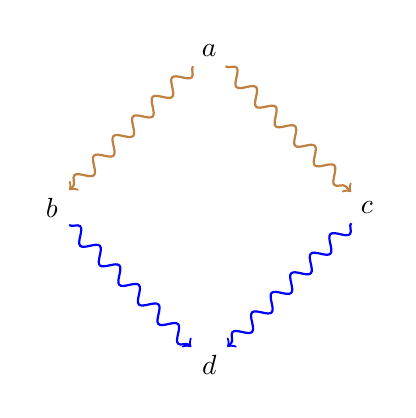
\begin{tikzpicture}
        \node (a)   at (2,4)  [circle] {$a$};
        \node (b)   at (0,2)  [circle] {$b$};
        \node (c)   at (4,2)  [circle] {$c$};
        \node (d)   at (2,0)  [circle] {$d$};

        \draw[->, thick, draw=brown, decorate, decoration=snake] (a) to (b);
        \draw[->, thick, draw=brown, decorate, decoration=snake] (a) to (c);
        \draw[->, thick, draw=blue,  decorate, decoration=snake] (b) to (d);
        \draw[->, thick, draw=blue,  decorate, decoration=snake] (c) to (d);
    \end{tikzpicture}
    \caption{Confluence}
    \label{fig:confluence.tikz}
\end{figure}

The next theorem shows that confluence is all we need to reduce the relation $\leftrightarrow^*$
to the relation $\rightarrow^*$. 

\begin{Theorem}[Church-Rosser]
  If the relation $\rightarrow \;\subseteq\; M \times M$ is confluent, then we have
  \\[0.2cm]
  \hspace*{1.3cm}
  $\forall a, b \in M:\bigl( a \leftrightarrow^* b \;\Leftrightarrow\;
   \exists c \in M: (a \rightarrow^* c \;\wedge b \rightarrow^* c)\bigr)$.
 \end{Theorem}

 \proof
If $a \leftrightarrow^* b$ then there is a finite sequence $(s_k)_{k\in \{0,\cdots,n\}}$ such that
\\[0.2cm]
\hspace*{1.3cm}
$a = s_0 \leftrightarrow s_1 \leftrightarrow \cdots \leftrightarrow s_{n-1} \leftrightarrow s_n = b$.
\\[0.2cm]
We prove by induction on $n$ that there is an element $c \in M$ such that both $a \rightarrow^* c$ and
$b \rightarrow^* c$ holds.
\begin{description}
\item[Base Case:] $n = 0$.
  
      Then we have $a = b$ and we can define $c := a$.
\item[Induction Step:] $n \mapsto n+1$
      
      We have $a = s_0 \leftrightarrow s_1 \leftrightarrow \cdots \leftrightarrow s_{n} \leftrightarrow s_{n+1} = b$.
      By induction hypotheses we know that there exists a $d \in M$ such that
      \\[0.2cm]
      \hspace*{1.3cm}
      $a \rightarrow^* d$ \quad and \quad $s_{n} \rightarrow^* d$ 
      \\[0.2cm]
      hold.  Furthermore, we either have
      \\[0.2cm]
      \hspace*{1.3cm}
      $s_{n} \rightarrow b$ \quad or \quad $b \rightarrow s_{n}$.
      \\[0.2cm]
      We discuss these cases one by one.
      \begin{enumerate}
      \item Case: $s_n \rightarrow b$.

        Since we also have $s_{n} \rightarrow^* d$, the confluence of the relation $\rightarrow$ shows that
        there is an element $c \in M$ such 
        \\[0.2cm]
        \hspace*{1.3cm}
        $b \rightarrow^* c$ \quad and \quad $d \rightarrow^* c$ 
        \\[0.2cm]
        holds.  From $a \rightarrow^* d$ and $d \rightarrow^* c$ we have that $a \rightarrow^* c$.  Since we already
        know that $b \rightarrow^* c$, the proof is complete in this case. 
      \item Case: $b \rightarrow s_n$.

        Since we have $b \rightarrow s_n$ and $s_n \rightarrow^* d$, we can conclude
        $b \rightarrow^* d$.  Since we also have $a \rightarrow^* d$, the proof is
        complete if we define $c := d$.  \qed
      \end{enumerate}
\end{description}
In general, it is hard to prove that a relation $\rightarrow$ is confluent.  Things get easier if the relation
$\rightarrow$ is well-founded, since then there is a weaker notion than confluence that is already sufficient
to guarantee confluence.

\begin{Definition}[Local Confluence] \hspace*{\fill} \\
  The relation $\rightarrow \;\subseteq\; M \times M$ is \blue{locally confluent} iff the following holds:
  \\[0.2cm]
  \hspace*{1.3cm}
  $\forall a, b, c \in M: \bigl(a \rightarrow b \;\wedge\; a \rightarrow c \quad\Rightarrow\quad
   \exists d \in M: (b \rightarrow^* d \;\wedge\; c \rightarrow^* d)\bigr)
  $  \eox
\end{Definition}

\noindent
Figure \ref{fig:local-confluence.tikz} shows a diagram picturing the notion of local confluence.
Here, the relation $\rightarrow^*$ is denoted by a snakelike arrow.
\begin{figure}[!ht]
    \centering
    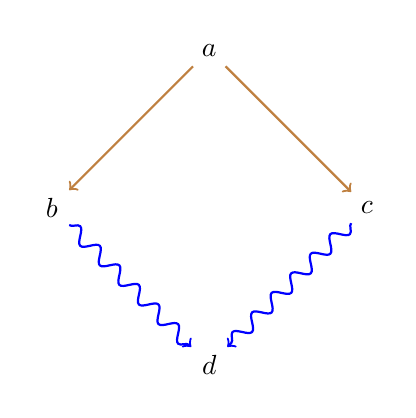
\begin{tikzpicture}
        \node (a)   at (2,4)  [circle] {$a$};
        \node (b)   at (0,2)  [circle] {$b$};
        \node (c)   at (4,2)  [circle] {$c$};
        \node (d)   at (2,0)  [circle] {$d$};

        \draw[->, thick, draw=brown] (a) to (b);
        \draw[->, thick, draw=brown] (a) to (c);
        \draw[->, thick, draw=blue,  decorate, decoration=snake] (b) to (d);
        \draw[->, thick, draw=blue,  decorate, decoration=snake] (c) to (d);
    \end{tikzpicture}
    \caption{Local Confluence}
    \label{fig:local-confluence.tikz}
\end{figure}

\begin{Theorem}[\href{https://en.wikipedia.org/wiki/Transfinite_induction}{Transfinite Induction}]
  \hspace*{\fill} \index{transfinite induction}\\
  Assume the relation $\rightarrow \;\subseteq\; M \times M$ is well-founded and $F(x)$ is some formula.
  If we have that
  \\[0.2cm]
  \hspace*{1.3cm}
  $\forall b \in M: \bigl( a \rightarrow^+ b \;\Rightarrow\; F(b)\bigr) \;\Rightarrow\; F(a)$ holds for all $a \in M$, \hspace*{\fill} (TI)
  \\[0.2cm]
  then we can conclude that $\forall a \in M: F(a)$ holds.
\end{Theorem}

\proof
Above, $\rightarrow^+$ denotes the transitive closure of $\rightarrow$.  We call $b$ a \blue{successor} of $a$
if $a \rightarrow^+ b$ holds.  The proof principle of transfinite induction is correct for a well-founded
relation because, first, if $a$ has no successors $b$, then the premise of (TI) which is
\\[0.2cm]
\hspace*{1.3cm}
$\forall b \in M: \bigl( a \rightarrow^+ b \Rightarrow F(b)\bigr)$
\\[0.2cm]
is vacuously true and hence by (TI) we know that $F(a)$ has to be true for all $a \in M$ that have no
successors.  Now assume $F(a)$ were false for some $a \in M$.  Then there must be a successor $a_1$ of $a$ such
that $F(a_1)$ is false because otherwise $F(a)$ would be true.  But then there must be a successor $a_2$ of
$a_1$ such that $F(a_2)$ is false.  Proceeding in this way we can construct an infinite sequence
\\[0.2cm]
\hspace*{1.3cm}
$a \rightarrow^+ a_1 \rightarrow^+ a_2 \rightarrow^+ \cdots \rightarrow^+ a_n \rightarrow^+ a_{n+1} \rightarrow
\cdots
$
\\[0.2cm]
such that $F(a_n)$ is false.  But this would contradict the well-foundedness of the relation $\rightarrow$.  Hence there can be no $a \in M$
such that $F(a)$ is false. \qed

\begin{Theorem}[\href{https://en.wikipedia.org/wiki/Newman\%27s_lemma}{Newman's Lemma}] \hspace*{\fill} \\
  If the relation $\rightarrow \;\subseteq\; M \times M$ is well-founded and locally confluent, then it is
  already confluent.
\end{Theorem}

\proof
Given any $a \in M$, we define the following formula:
\\[0.2cm]
\hspace*{1.3cm}
$F(a) \;:=\; \forall b, c \in M: \bigl(a \rightarrow^* b \;\wedge\; a \rightarrow^*c \quad\Rightarrow\quad
 \exists d \in M: (b \rightarrow^* d \;\wedge\; c \rightarrow^* d)\bigr)
$
\\[0.2cm]
We  prove that $F(a)$ holds for all $a \in M$ by transfinite induction.
Therefore, in order to prove $F(a)$ we may assume that $F(b)$ already holds for all successors $b$ of $a$.
So let us assume that we have
\\[0.2cm]
\hspace*{1.3cm}
$a \rightarrow^* b$ \quad and \quad $a \rightarrow^* c$.
\\[0.2cm]
We have to find an element $d \in M$ such that both $b \rightarrow^* d$ and $c \rightarrow^* d$ holds.
Now since $a \rightarrow^* b$, either $a = b$ or there is an element $b_1$ such that
\\[0.2cm]
\hspace*{1.3cm}
$a \rightarrow b_1 \rightarrow^* b$
\\[0.2cm]
holds.  If $a = b$ we can define $d := c$ and because of $a \rightarrow^* c$ we would then have both
\\[0.2cm]
\hspace*{1.3cm}
$b \rightarrow^* d$ \quad and \quad $c \rightarrow^* d$
\\[0.2cm]
and therefore, in the case $a = b$, we are done.  Similarly, since $a \rightarrow^* c$ we either have
$a = c$ or there is an element $c_1$ such that
\\[0.2cm]
\hspace*{1.3cm}
$a \rightarrow c_1 \rightarrow^* c$
\\[0.2cm]
holds.  If $a = c$ we can define $d := b$ and because of $a \rightarrow^* b$ we would then have both
\\[0.2cm]
\hspace*{1.3cm}
$b \rightarrow^* d$ \quad and \quad $c \rightarrow^* d$
\\[0.2cm]
and are done again.  Now the case that is left is the following:
\\[0.2cm]
\hspace*{1.3cm}
$a \rightarrow b_1 \rightarrow^* b$ \quad and \quad $a \rightarrow c_1 \rightarrow^* c$.
\\[0.2cm]
Since $\rightarrow$ is locally confluent and we have both $a \rightarrow b_1$ and  $a \rightarrow c_1$ 
there exists an element $d_1$ such that we have
\\[0.2cm]
\hspace*{1.3cm}
$b_1 \rightarrow^* d_1$ \quad and \quad $c_1 \rightarrow^* d_1$.
\\[0.2cm]
Now as $b_1$ is a successor of $a$ and we have both
\\[0.2cm]
\hspace*{1.3cm}
$b_1 \rightarrow^* b$ \quad and \quad $b_1 \rightarrow^* d_1$,
\\[0.2cm]
our induction hypotheses tells us that there is an element $d_2$ such that we have both
\\[0.2cm]
\hspace*{1.3cm}
$b \rightarrow^* d_2$ \quad and \quad $d_1 \rightarrow^* d_2$.
\\[0.2cm]
Now we have $c_1 \rightarrow^* d_1$ and $d_1 \rightarrow^* d_2$, which implies
\\[0.2cm]
\hspace*{1.3cm}
$c_1 \rightarrow^* d_2$
\\[0.2cm]
As we also have $c_1 \rightarrow^* c$ we have both
\\[0.2cm]
\hspace*{1.3cm}
$c_1 \rightarrow^* d_2$ \quad and \quad $c_1 \rightarrow^* c$.
\\[0.2cm]
Since $c_1$ is a successor of $a$, the induction hypotheses tells us that there is an element $d$ such that we
have both
\\[0.2cm]
\hspace*{1.3cm}
$d_2 \rightarrow^* d$ \quad and \quad $c \rightarrow^* d$.
\\[0.2cm]
As we have $b \rightarrow^* d_2$ and $d_2 \rightarrow^* d$ we can conclude $b \rightarrow^* d$.  Hence we have
\\[0.2cm]
\hspace*{1.3cm}
$b \rightarrow^* d$ \quad  and \quad $c \rightarrow^* d$
\\[0.2cm]
and the proof is complete.  Figure \ref{fig:newman.pdf} on page \pageref{fig:newman.pdf} shows how the
different elements are related and conveys the idea of the proof in a concise way. \qed

\begin{figure}[!ht]
  \centering
  \framebox{\epsfig{file=Figures/newman.pdf,scale=0.3}} 
  \caption{The Proof of Newman's Lemma.}
  \label{fig:newman.pdf}
\end{figure}

\section{The Knuth-Bendix Order}
In this section we define the \blue{Knuth-Bendix order} $\prec$ on the set $\mathcal{T}_\Sigma$ of
$\Sigma$-terms.  In order to do so, three prerequisites need to be satisfied:
\begin{enumerate}
\item We need to assign a \blue{weight} $w(f)$ to every function symbol $f$.  These weights are 
      natural numbers.  In addition, there must be at most one function symbol $g$ such that $w(g) = 0$.
      Furthermore, if $w(g) = 0$, then $g$ has to be unary.
\item We need to have a \blue{strict total order} $<$ on the set of function symbols, i.e. the following
      conditions need to be satisfied:
      \begin{enumerate}[(a)]
      \item The relation $<$ is \blue{irreflexive}, that is we have $\neg (f < f)$ for all function symbols $f$.
      \item The relation $<$ is \blue{transitive}, that is we have 
            \\[0.2cm]
            \hspace*{1.3cm}
            $f < g \wedge g < h \Rightarrow f < h$ \quad for all function symbols $f$, $g$, and $h$.
      \item The relation $<$ is \blue{total}, that is we have 
            \\[0.2cm]
            \hspace*{1.3cm}
            $f < g \,\vee\, f = g \,\vee\, g < f$ \quad for all function symbols $f$ and $g$.
      \end{enumerate}
\item The order $<$ on the function symbols has to be \blue{admissible} with respect to the weight function
      $w$, i.e. the following condition needs to be satisfied:
   $$ w(f) = 0 \rightarrow \forall g:  \bigl(g \not=f \rightarrow g < f\bigr). $$
      To put this in words: If the function symbol $f$ has a weight of $0$, then 
      all other function symbols $g$ have to be smaller than $f$ w.r.t.~the strict order $<$.
      Note that this implies that there can be at most one function symbol with $f$ such that $w(f) = 0$. 
      This function symbol $f$ is then the maximum w.r.t.~the order $<$.
\end{enumerate}
Given the function $w$ that assigns a weight to all function symbols, we can define the \blue{weight} $w(t)$ of a
$\Sigma$-term $t$ by induction on $t$.
\begin{enumerate}
\item $w(x) := 1$ for all variables $x$,
\item $w\bigl(f(t_1,\cdots,t_n)\bigr) := w(f) + \sum\limits_{i=1}^n w(t_i)$.
\end{enumerate}
Furthermore, we define the function
\\[0.2cm]
\hspace*{1.3cm}
$\texttt{count}: \mathcal{T}_\Sigma \times \mathcal{V} \rightarrow \mathbb{N}$
\\[0.2cm]
that takes a term $t$ and a variable $x$ and returns the number of times that $x$ occurs in $t$.
We define $\texttt{count}(t,x)$ by induction on $t$.
\begin{enumerate}
\item $\texttt{count}(x, x) := 1$ for every variable $x \in \mathcal{V}$.
\item $\texttt{count}(y, x) := 0$ if $x \not= y$ for all variables $x,y \in \mathcal{V}$.
\item $\texttt{count}\bigl(f(t_1,\cdots,t_n), x\bigr) := \sum\limits_{i=1}^n \texttt{count}(t_i, x)$.
\end{enumerate}
Now we are ready to define the \blue{Knuth-Bendix order}.  Given two terms $s$ and $t$  
we have $s \prec t$ iff one of the following two conditions hold:
\begin{enumerate}
\item $w(s) < w(t)$ and $\texttt{count}(s, x) \leq \texttt{count}(t, x)$
       for all variables $x$ occurring in  $s$.
\item $w(s) = w(t)$, $\texttt{count}(s, x) \leq \texttt{count}(t, x)$ for all variables $x$ occuring in $s$, and
      one of the following subconditions holds:
      \begin{enumerate}[(a)]
      \item $t = f^n(s)$ where $n \geq 1$ and $f$ is the maximum w.r.t.~the order $<$ on function symbols,
             i.e.~we have $g < f$ for all function symbols $g \not= f$.
      \item $s = f(s_1,\cdots,s_m)$, $t=g(t_1,\cdots,t_n)$, and $f<g$.
      \item $s = f(s_1,\cdots,s_m)$, $t=f(t_1,\cdots,t_m)$, and $[s_1,\cdots,s_m] \prec_{\textrm{lex}} [t_1,\cdots,t_m]$.
     
            Here, $\prec_{\textrm{lex}}$ denotes the \blue{lexicographic extension} of the ordering $\prec$ to
            lists of terms.  It is defined as follows:
            $$ [x] + R_1 \prec_{\textrm{lex}} [y] + R_2 \;\stackrel{_\textrm{def}}{\Longleftrightarrow}\;
                 x \prec y \,\vee\, \bigl(x = y \wedge R_1 \prec_{\textrm{lex}} R_2\bigr)
            $$
     \end{enumerate}
\end{enumerate}

\begin{Theorem}
  The Knuth-Bendix order is a rewrite order.
\end{Theorem}

Proving that the Knuth-Bendix order is a strict partial order on the set $\mathcal{T}_\Sigma$ that is stable
and a congruence can be done via induction on the structure of the terms.  The hard part of the proof is to
show that the Knuth-Bendix order is well-founded.  A proof is given in the book by Franz Baader and Tobias
Nipkow \cite{baader:1998}.

\section{Unification}
This section introduces the notion of a \blue{most general unifier} of two terms.
To begin, we define the composition of two $\Sigma$-substitutions.

\begin{Definition}[Composition of Substitutions] \index{Composition von Substitutions}
    Assume that \\[0.2cm]
    \hspace*{1.3cm}
    $\sigma = \{ x_1 \mapsto s_1, \cdots, x_m \mapsto s_m \}$
    \quad and \quad
    $\tau = \{ y_1 \mapsto t_1, \cdots, y_n \mapsto t_n \}$
    \\[0.2cm]
    are two substitutions such that $\textsl{dom}(\sigma) \cap \textsl{dom}(\tau) = \{\}$.
    We define the  \blue{composition $\sigma\tau$} \index{composition $\sigma\tau$} of $\sigma$ and $\tau$  as
    \\[0.2cm]
    \hspace*{1.3cm}
    $\sigma\tau := \{ x_1 \mapsto s_1\tau, \cdots, x_m \mapsto s_m\tau,\; y_1 \mapsto t_1, \cdots, y_n \mapsto t_n \}$
    \eox
\end{Definition}

\example
If we define
\\[0.2cm]
\hspace*{1.3cm}
$\sigma := \{ x_1 \mapsto c,\; x_2 \mapsto f(x_3) \}$ \quad and \quad
$\tau := \{ x_3 \mapsto h(c,c),\; x_4 \mapsto d \}$,
\\[0.2cm]
then we have
\\[0.2cm]
\hspace*{1.3cm}
$\sigma\tau = \{ x_1 \mapsto c,\; x_2 \mapsto f(h(c,c)),\; x_3 \mapsto h(c,c),\;x_4 \mapsto d \}$.
\eoxs
\vspace{0.3cm}

\begin{Proposition} \label{satz:composition}
    If $t$ is a term and $\sigma$ and $\tau$ are substitutions such that  
    $\textsl{dom}(\sigma) \cap \textsl{dom}(\tau) = \{\}$ holds, then we have
    \\[0.2cm]
    \hspace*{1.3cm} $(t \sigma)\tau = t (\sigma\tau)$.
    \eoxs
\end{Proposition}
This proposition may be proven by induction on $t$.

\begin{Definition}[Syntactical Equation] \index{syntactical equation}
  A  \blue{syntactical equation} is a pair $\langle s, t \rangle$ of terms.
  It is written as $s \doteq t$. \index{$s \doteq t$}
  A \blue{system of syntactical equations} \index{system of syntactical equations} is a set of syntactical
  equations.
  \eoxs
\end{Definition}


\begin{Definition}[Unifier]
  A substitution $\sigma$ \blue{solves} a syntactical equation $s \doteq t$ iff we have $s\sigma = t\sigma$.
  If $E$ is a system of syntactical equations and $\sigma$ is a substitution that solves
  every syntactical equations in $E$, then $\sigma$ is a  \blue{unifier} \index{unifier} of $E$.
  \eoxs
\end{Definition}

\noindent
If $E = \{ s_1 \doteq t_1, \cdots, s_n \doteq t_n \}$ is a system of syntactical equations and $\sigma$ is a
substitution, then we define
\\[0.2cm]
\hspace*{1.3cm}  $E\sigma := \{ s_1\sigma \doteq t_1\sigma, \cdots, s_n\sigma \doteq t_n\sigma \}$.
\vspace{0.3cm}

\example
Let us consider the syntactical equation
\\[0.2cm]
\hspace*{1.3cm}
$p(x_1, f(x_4)) \doteq p( x_2, x_3)$
\\[0.2cm]
and define the substitution
\\[0.2cm]
\hspace*{1.3cm}
$\sigma := \{ x_1 \mapsto x_2,\; x_3 \mapsto f(x_4) \}$.
\\[0.2cm]
Then $\sigma$ solves the given syntactical equation because we have
\\[0.2cm]
\hspace*{1.3cm}
$p(x_1, f(x_4))\sigma = p(x_2, f(x_4))$ \quad und \quad \\[0.2cm]
\hspace*{1.3cm}
$p(x_2, x_3)\sigma \;\quad = p(x_2, f(x_4))$.  \eox

Next we develop an algorithm for solving a system of syntactical equations.
The algorithm we present was published by Martelli and Montanari
\cite{martelli:1982}.\index{algorithm of Martelli and Montanari}  
To begin, we first consider the cases where a syntactical equation $s \doteq t$ is \blue{unsolvable}.
There are two cases: A syntactical equation of the form
\\[0.2cm]
\hspace*{1.3cm}
$f(s_1,\cdots,s_m) \doteq g(t_1,\cdots, t_n)$ \\[0.2cm]
is certainly unsolvable if  $f$ and $g$ are different function symbols. The reason is that for any substitution
$\sigma$ we have that \\[0.2cm]
\hspace*{1.0cm} $f(s_1,\cdots,s_m)\sigma = f(s_1\sigma,\cdots,s_m\sigma)$ \quad und \quad
                $g(t_1,\cdots, t_n)\sigma = g(t_1\sigma,\cdots,t_n\sigma)$. \\[0.2cm]
If $f \not = g$, then the terms  $f(s_1,\cdots,s_m)\sigma$ and $g(t_1,\cdots, t_n)\sigma$ start with different
function symbols and hence they can't be identical.

The other case where a syntactical equation is unsolvable, is a syntactical equation of the following form:
\\[0.2cm]
\hspace*{1.3cm}
$x \doteq f(t_1,\cdots,t_n)$  \quad where $x \in \texttt{var}\big(f(t_1,\cdots,t_n)\big)$.
\\[0.2cm]
This syntactical equation is unsolvable because the term $f(t_1,\cdots,t_n)\sigma$ will always contain at least one more
occurrence of the function symbol $f$ than the term $x\sigma$.

Now we are able to present an algorithm for solving a system of syntactical equations, provided the system is
solvable.  The algorithm will also discover if a system of syntactical equations is unsolvable.
The algorithm works on pairs of the form
$\langle F, \tau \rangle$ where $F$ is a system of syntactical equations and $\tau$ is a substitution.
The algorithm starts with the pair 
$\langle E, \{\} \rangle$.  Here $E$ is the system of syntactical equations that is to be solved and $\{\}$
represents the empty substitution.  The system works by simplifying the pairs $\langle F, \tau \rangle$ using
certain reduction rules that are presented below.  These reduction rules are applied until we either discover
that the system of syntactical equations is unsolvable or else we reduce the pairs until we finally arrive at a
pair of the form $\langle \{\}, \mu \rangle$.  In this case  $\mu$ is a unifier of the system of
syntactical equations $E$.  The reduction rules are as follows:
\begin{enumerate}
\item If  $y\in\mathcal{V}$ is a variable that does  \underline{\color{red}not} occur in the term $t$, then
      we can perform the following reduction: 
      \[ \Big\langle E \cup \big\{ y \doteq t \big\}, \sigma \Big\rangle \quad\leadsto\quad 
         \Big\langle E\{y \mapsto t\}, \sigma\{ y \mapsto t \} \Big\rangle \qquad\mbox{if $y \in \mathcal{V}$
           and $y \not\in \mathtt{var}(t)$} 
      \]
      This reduction rule can be understood as follows: If the system of syntactical equations that is to be
      solved contains a syntactical equation of the form $y \doteq t$, where the variable $y$ does not occur in
      the term $t$, then the syntactical equation $y \doteq t$ can be removed if we apply the substitution
      $\{ y \mapsto t \}$ to both components of the pair
      \\[0.2cm]
      \hspace*{1.3cm}
      $\Big\langle E \cup \big\{ y \doteq t \big\}, \sigma \Big\rangle$.
\item If the variable $y$ occurs in the term $t$, i.e.~if  $y \in \textsl{Var}(t)$
      and, furthermore, $t \not= y$, then the system of syntactical equations
      $E \cup \big\{ y \doteq t \big\}$ has no solution.  We write this as
      \\[0.2cm]
      \hspace*{1.3cm}
      $\Big\langle E \cup \big\{ y \doteq t \big\}, \sigma \Big\rangle\;\leadsto\; \Omega$ \quad
      if $y \in \texttt{var}(t)$ and $y \not=t$.
\item If $y\in\mathcal{V}$ and  $t \not\in \mathcal{V}$, then we have:
      \[ \Big\langle E \cup \big\{ t \doteq y \big\}, \sigma \Big\rangle \quad\leadsto\quad 
         \Big\langle E \cup \big\{ y \doteq t \big\}, \sigma \Big\rangle \qquad\mbox{if $y \in \mathcal{V}$ and
           $t \not\in \mathcal{V}$.}
      \]   
      After we apply this rule, we can apply either the first or the second reduction rule thereafter.
\item Trivial syntactical equations can be deleted:
      \[ \Big\langle E \cup \big\{ x \doteq x \big\}, \sigma \Big\rangle \quad\leadsto\quad
         \Big\langle E, \sigma \Big\rangle \qquad\mbox{if $x \in \mathcal{V}$.}
      \]   
\item If $f$ is an  $n$-ary function symbol we have 
      \[ \Big\langle E \cup \big\{ f(s_1,\cdots,s_n) \doteq f(t_1,\cdots,t_n) \big\}, \sigma \Big\rangle 
         \;\leadsto\; 
         \Big\langle E \cup \big\{ s_1 \doteq t_1, \cdots, s_n \doteq t_n\}, \sigma \Big\rangle.
      \]   

      This rule is the reason that we have to work with a system of syntactical equations, because even if we
      start with a single syntactical equation the rule given above can increase the number of syntactical
      equations. 

      A special case of this rule is the following:  
      \[ \Big\langle E \cup \big\{ c \doteq c \big\}, \sigma \Big\rangle \;\leadsto\; 
         \Big\langle E, \sigma \Big\rangle.
      \]
      Here $c$ is a nullary function symbol.
\item The system of syntactical equations $E \cup \big\{ f(s_1,\cdots,s_m) \doteq g(t_1,\cdots,t_n) \big\}$ has
      no solution if the function symbols $f$ and $g$ are different.  Hence we have
      \[ \Big\langle E \cup \big\{ f(s_1,\cdots,s_m) \doteq g(t_1,\cdots,t_n) \big\},
      \sigma \Big\rangle \;\leadsto\; \Omega \qquad \mbox{provided $f \not= g$}. \]
\end{enumerate}
If a system of syntactical equations $E$ is given and we start with the pair 
$\langle E, \{\}\rangle$, then we can apply the rules given above until one of the following two cases happens: 
\begin{enumerate}
\item We use the second or the sixth of the reduction rules given above.
      In this case the system of syntactical equations $E$ is unsolvable.
\item The pair $\langle E, \{\} \rangle$ is reduced into a pair of the form $\langle \{\}, \mu\rangle$.
      Then $\mu$ is a  \blue{unifier} of $E$.  In this case we write $\mu = \mathtt{mgu}(E)$.
      If $E = \{ s \doteq t \}$, we write $\mu = \mathtt{mgu}(s, t)$.  The abbreviation
      $\mathtt{mgu}$ is short for {``\blue{most general unifier}''}.
\end{enumerate}

\example
We show how to solve the syntactical equation \\[0.2cm]
\hspace*{1.3cm}  $p(x_1, f(x_4)) \doteq p( x_2, x_3)$.  \\[0.2cm]
We have the following reductions:
$$
\begin{array}{ll}
          &  \big\langle \big\{ p(x_1, f(x_4)) \doteq p( x_2, x_3) \big\}, \{ \} \big\rangle \\[0.2cm]
 \leadsto &  \big\langle \big\{ x_1 \doteq x_2, f(x_4) \doteq x_3 \big\}, \{ \} \big\rangle \\[0.2cm]
 \leadsto &  \big\langle \big\{ f(x_4) \doteq x_3 \big\}, \{ x_1 \mapsto x_2 \} \big\rangle \\[0.2cm]
 \leadsto &  \big\langle \big\{ x_3 \doteq f(x_4) \big\}, \{ x_1 \mapsto x_2 \} \big\rangle \\[0.2cm]
 \leadsto &  \big\langle \big\{\big\}, \{ x_1 \mapsto x_2,\; x_3 \mapsto f(x_4) \} \big\rangle \\[0.2cm]
\end{array}
$$
Hence the method is successful and we have that the substitution
\\[0.2cm]
\hspace*{1.3cm}
$\{ x_1 \mapsto x_2,\; x_3 \mapsto f(x_4) \}$ \\[0.2cm]
is a solution of the syntactical equation given above.  \eox

\example
Next we try to solve the following system of syntactical equations: 
\[ E = \big\{ p(h(x_1,c)) \doteq p(x_2),\; q(x_2, d) \doteq q(h(d,c),x_4) \big\} \]
We have the following reductions:
$$
\begin{array}{ll}
          & \big\langle \big\{ p(h(x_1,c)) \doteq p(x_2),\; q(x_2, d) \doteq q(h(d,c),x_4) \big\}, \{ \} \big\rangle \\[0.2cm]
 \leadsto & \big\langle \big\{ p(h(x_1,c)) \doteq p(x_2),\; x_2 \doteq h(d,c), \; d \doteq x_4 \big\}, \{ \} \big\rangle \\[0.2cm]
 \leadsto & \big\langle \big\{ p(h(x_1,c)) \doteq p(x_2),\; x_2 \doteq h(d,c), \; x_4 \doteq d \big\}, \{ \} \big\rangle \\[0.2cm]
 \leadsto & \big\langle \big\{ p(h(x_1,c)) \doteq p(x_2),\; x_2 \doteq h(d,c) \big\}, \{ x_4 \mapsto d \} \big\rangle \\[0.2cm]
 \leadsto & \big\langle \big\{ p(h(x_1,c)) \doteq p(h(d,c)) \big\}, \{ x_4 \mapsto d,\; x_2 \mapsto h(d,c) \} \big\rangle \\[0.2cm]
 \leadsto & \big\langle \big\{ h(x_1,c) \doteq h(d,c) \big\}, \{ x_4 \mapsto d,\; x_2 \mapsto h(d,c) \} \big\rangle \\[0.2cm]
 \leadsto & \big\langle \big\{ x_1 \doteq d,\; c \doteq c \big\}, \{ x_4 \mapsto d,\; x_2 \mapsto h(d,c) \} \big\rangle \\[0.2cm]
 \leadsto & \big\langle \big\{ x_1 \doteq d,\big\}, \{ x_4 \mapsto d,\; x_2 \mapsto h(d,c) \} \big\rangle \\[0.2cm]
 \leadsto & \big\langle \big\{\big\}, \{ x_4 \mapsto d,\; x_2 \mapsto h(d,c),\; x_1 \mapsto d \} \big\rangle \\[0.2cm]
\end{array}
$$
Hence the  substitution  $\{ x_4 \mapsto d,\; x_2 \mapsto h(d,c),\; x_1 \mapsto d \}$ is a solution
of the system of syntactical equations given above.
\eox


\section{The Knuth-Bendix Algorithm}
Assume we have been given a set $R$ of rewrite rules such that
\\[0.2cm]
\hspace*{1.3cm}
$r \prec l$ \quad holds for all $l \approx r$ in $R$
\\[0.2cm]
such that the relation $\prec$ is a rewrite order.
Given two terms $s$ and $t$, the Church-Rosser Theorem tells us, that we can decide the question whether
$s \leftrightarrow_R^* t$ holds by rewriting $s$ and $t$ into normal forms, provided the relation
$\rightarrow_R$ is confluent.  By Newman's Lemma we know that local confluence is sufficient.  Donald E.~Knuth
and Peter B.~Bendix \cite{knuth:1970} have discovered a way to decide whether the term rewriting relation
$\rightarrow_R$ is locally confluent.  To understand their idea, we introduce the notion of a \blue{critical pair}.

\begin{Definition}[Critical Pair] \hspace*{\fill} \\
  \index{critical pair}
  Assume we have been given the equations $l_1 \approx r_1$ and $l_2 \approx r_2$.  These equations
  \blue{generate} a critical pair if and only if all of the following conditions hold:
  \begin{enumerate}[(a)]
  \item There exists a position $u \in \Pos(l_1)$ such that $l_1/u$ is not a variable.
  \item The subterm $l_1/u$ of $l_1$ is unifiable with $l_2$.  For the following, assume that $\mu$ is a most general unifier
        of $l_1/u$ and $l_2$, i.e.~we have
        \\[0.2cm]
        \hspace*{1.3cm}
        $\mu = \texttt{mgu}(l_1/u, l_2)$.
  \item The term $s$ results from rewriting the term $l_1\mu$ by rewriting the subterm $l_1\mu/u$
        to the new subterm $r_2\mu$ using the rewrite rule $l_2 \approx r_2$:      
        \\[0.2cm]
        \hspace*{1.3cm}
        $s = l_1\mu[u \mapsto r_2\mu]$.
  \item The term $t$ results from rewriting the term $l_1\mu$ into the term $r_1\mu$ using the rule
        $l_1 \approx r_1$, i.e.~we have
        \\[0.2cm]
        \hspace*{1.3cm}
        $t = r_1\mu$.  
      \end{enumerate}
      Then the pair $\langle s, t \rangle$, which is
      \\[0.2cm]
      \hspace*{1.3cm}
      $\bigl\langle l_1\mu[u \mapsto r_2\mu],\; r_1\mu \bigr\rangle$
      \\[0.2cm]
      is a \blue{critical pair} of $l_1 \approx r_1$ and $l_2 \approx r_2$. \eod
\end{Definition}

\example
The following example assumes the signature $\Sigma_G$ from group theory as given.
We start with the two equations $(x \circ y) \circ z \approx x \circ (y \circ z)$ and $i(w) \circ w \approx e$.
Then $u = [1]$ is a position in the term $(x \circ y) \circ z$ and we have
\\[0.2cm]
\hspace*{1.3cm}
$\bigl((x \circ y) \circ z\bigr)/[1] = x \circ y$, which is not a variable.
\\[0.2cm]
The term $x \circ y$ can be unified with the term $i(w) \circ w$ and we have
\\[0.2cm]
\hspace*{1.3cm}
$\mu := \texttt{mgu}\bigl(x \circ y, i(w) \circ w\bigr) = \{ x \mapsto i(w),\; y \mapsto w \}$.
\\[0.2cm]
Therefore we have
\\[0.2cm]
\hspace*{1.3cm}
$\bigl((x \circ y) \circ z\bigr)\mu = \bigl(i(w) \circ w\bigr) \circ z$
\\[0.2cm]
and the latter term can be rewritten by the equation $i(w) \circ w \approx e$ into the term $e \circ z$,
i.e.~we have
\\[0.2cm]
\hspace*{1.3cm}
$\bigl(i(w) \circ w\bigr) \circ z \rightarrow_{\{ i(w) \circ w \approx e\}} e \circ z$.
\\[0.2cm]
Furthermore, the same term $\bigl(i(w) \circ w\bigr) \circ z$ can be rewritten by the equation
$(x \circ y) \circ z \approx x \circ (y \circ z)$ into the term $i(w) \circ (w \circ z)$:  
\\[0.2cm]
\hspace*{1.3cm}
$\bigl(i(w) \circ w\bigr) \circ z \rightarrow_{\{ (x \circ y) \circ z \approx x \circ (y \circ z)\}} i(w) \circ (w \circ z)$.
\\[0.2cm]
Therefore, the pair
\\[0.2cm]
\hspace*{1.3cm}
$\bigl\langle e \circ z,\; i(w) \circ (w \circ z) \bigr\rangle$
\\[0.2cm]
is a critical pair of the two equations  $(x \circ y) \circ z \approx x \circ (y \circ z)$ and $i(w) \circ w \approx e$.
\eox

\remark
If $\langle s, t\rangle$ is a critical pair from two equations in a set $R$, then the equation $s \approx t$
follows from $R$, i.e.~we have
\\[0.2cm]
\hspace*{1.3cm}
$R \models s \approx t$. \eox


\begin{Definition}[Confluent Critical Pair] \hspace*{\fill} \\
  A critical pair $\langle s_1, s_2\rangle$ is \blue{confluent} w.r.t.~a rewrite relation $R$ iff there is a term
  $t$ such that $t$ is in $R$-normal form and we have both
  \\[0.2cm]
  \hspace*{1.3cm}
  $s_1 \rightarrow^*_R t$ \quad and \quad   $s_2 \rightarrow^*_R t$.  
\end{Definition}

\begin{Theorem}[Knuth-Bendix]
  If $R$ is a set of rewrite equations such that all critical pairs between equations from $R$ are confluent,
  then the rewrite relation $\rightarrow^*_R$ is confluent and hence the question, whether $R \models s \approx t$
  can be decided by rewriting both $s$ and $t$ into normal forms $\widehat{s}$ and $\widehat{t}$:
  \\[0.2cm]
  \hspace*{1.3cm}
  $s \rightarrow^*_R \widehat{s}$ \quad and \quad  $t \rightarrow^*_R \widehat{t}$ 
  \\[0.2cm]
  Then we have
  \\[0.2cm]
  \hspace*{1.3cm}
  $R \models s \approx t$ \quad if and only if \quad $\widehat{s} = \widehat{t}$.
\end{Theorem}

\noindent
To make the above theorem work, if we start with a set $E$ of equations, we first have to order them into a set
of rewrite rules $R$.  In general, this will not be sufficient because there will be critical pairs that are
not confluent. However, if we can orient these newly derived critical pairs into new rewrite rules, we might be
able to extend the set $R$ to a new set of rewrite $\widehat{R}$ such that all critical pairs from equations
from $\widehat{R}$ are confluent.
\vspace*{0.2cm}

\noindent
\textbf{Knuth-Bendix Algorithm}:  Given a set of equations $E$ the Knuth-Bendix algorithm proceeds as follows:
\begin{enumerate}
\item We define suitable weight for the function symbols occurring in $E$ and order the function symbols
      such that every equation  $(s \approx t) \in E$ can be ordered as either $s \prec t$ or $t \prec s$.
      If this is not possible, the algorithm fails.
\item Otherwise, call $R$ the set of oriented rewrite rules that result from orienting the equations in $E$
      into rewrite rules.
\item Compute all critical pairs that can be build from equations in $R$.
      \begin{enumerate}
      \item If all critical pairs are confluent, then the rewrite relation $\rightarrow^*_R$ is confluent
            and the algorithm is successful.
      \item If we have found a critical pair $\langle s, t \rangle$ that is not confluent,
            we orient the equation $s \approx t$ into a rewrite rule.  If this is impossible, the algorithm fails.
            Otherwise, we add the oriented equation to $R$.
            Now the set $R$ could generate additional critical pairs.
            Hence we must go back to the beginning of step 3. \eod
      \end{enumerate}
\end{enumerate}

\noindent
The algorithm shown above can have three different outcomes:
\begin{enumerate}
\item It can fail because it has generated an equation that can not be oriented into a rewrite rule.
\item It can stop with a set of rewrite rules $R$ such that $\rightarrow_R$ is confluent.
\item It can run forever because an infinite set of critical pairs is generated.
\end{enumerate} 
My GitHub repository contains the Jupyter notebook
\\[0.2cm]
\hspace*{1.3cm}
\href{https://github.com/karlstroetmann/Artificial-Intelligence/blob/master/Python/4%20Automatic%20Theorem%20Proving/Knuth-Bendix-Algorithm-KBO.ipynb}{Knuth-Bendix-Algorithm-KBO.ipynb}
\\[0.2cm]
which contains an implementation of the Knuth-Bendix algorithm.  It also contains a number of equational
theories $E$ where the Knuth-Bendix algorithm is successful.

\example
We test the Knuth-Bendix algorithm with the axioms of group theory.  These axioms are the following:
\begin{enumerate}[(a)]
\item $1 \circ x \approx x$,
\item $i(x) \circ x \approx 1$, and
\item $(x \circ y) \circ z \approx x \circ (y \circ z)$.
\end{enumerate}
It is obvious how these equations can be oriented into rewrite rules.  The resulting rules are:
\begin{itemize}
\item $1 \circ x \rightarrow x$,
\item $i(x) \circ x \rightarrow 1$, and
\item $(x \circ y) \circ z \rightarrow x \circ (y \circ z)$.
\end{itemize}
From $(x \circ y) \circ z \rightarrow x \circ (y \circ z)$ and  $i(a) \circ a \rightarrow 1$ we conclude
\\[0.2cm]
\hspace*{1.3cm}
$(i(a) \circ a) \circ z \rightarrow i(a) \circ (a \circ z)$ \quad and \quad
$(i(a) \circ a) \circ z \rightarrow 1 \circ z$
\\[0.2cm]
Hence we have found the new rewrite rule
\\[0.2cm]
\hspace*{1.3cm}
$i(a) \circ (a \circ z) \rightarrow z$.
\\[0.2cm]
From $i(a) \circ (a \circ z) \rightarrow z$ and $i(x) \circ x$ we conclude
\\[0.2cm]
\hspace*{1.3cm}
$i(i(x)) \circ (i(x) \circ x) \rightarrow x$ \quad and \quad
$i(i(x)) \circ (i(x) \circ x) \rightarrow i(i(x)) \circ 1$. 
\\[0.2cm]
Hence we have found the new rewrite rule
\\[0.2cm]
\hspace*{1.3cm}
$i(i(x)) \circ 1 \rightarrow x$.
\\[0.2cm]
From $i(x) \circ (x \circ y) \rightarrow y$ and $i(a) \circ (a \circ b) \rightarrow b$ we conclude
\\[0.2cm]
\hspace*{1.3cm}
$i\bigl(i(a)\bigr) \circ \bigl(i(a) \circ (a \circ b)\bigr) \rightarrow a \circ b $ \quad and \quad
$i\bigl(i(a)\bigr) \circ \bigl(i(a) \circ (a \circ b)\bigr) \rightarrow i\bigl(i(a)\bigr) \circ b$.
\\[0.2cm]
Hence we have found the new rewrite rule
\\[0.2cm]
\hspace*{1.3cm}
$i\bigl(i(a)\bigr) \circ b \rightarrow a \circ b$
\\[0.2cm]
From $i\bigl(i(a)\bigr) \circ b \rightarrow a \circ b$ and $i(i(x)) \circ 1 \rightarrow x$ we conclude
\\[0.2cm]
\hspace*{1.3cm}
$i\bigl(i(a)\bigr) \circ 1 \rightarrow a \circ 1$ \quad and \quad
$i\bigl(i(a)\bigr) \circ 1 \rightarrow a$
\\[0.2cm]
Hence we have found the new rewrite rule
\\[0.2cm]
\hspace*{1.3cm}
$a \circ 1 \rightarrow a$.
\\[0.2cm]
At this point, the rewrite rule $i\bigl(i(x)\bigr) \circ 1 \rightarrow x$ is simplified into the rule
\\[0.2cm]
\hspace*{1.3cm}
$i\bigl(i(x)\bigr) \rightarrow x$.
\\[0.2cm]
From $i(x) \circ (x \circ y) \rightarrow y$ and $i\bigl(i(a)\bigr) \rightarrow a$ we conclude
\\[0.2cm]
\hspace*{1.3cm}
$i\bigl(i(a)\bigr) \circ \bigl(i(a)\circ y\bigr) \rightarrow y$ \quad and \quad
$i\bigl(i(a)\bigr) \circ \bigl(i(a)\circ y\bigr) \rightarrow a \circ \bigl(i(a) \circ y\bigr)$.
\\[0.2cm]
Hence we have found the new rule
\\[0.2cm]
\hspace*{1.3cm}
$a \circ \bigl(i(a) \circ y\bigr) \rightarrow y$.
\\[0.2cm]
From $i(x) \circ x \rightarrow 1$ and $i\bigl(i(a)\bigr) \rightarrow a$ we conclude
\\[0.2cm]
\hspace*{1.3cm}
$i\bigl(i(a)\bigr) \circ i(a) \rightarrow 1$ \quad and \quad
$i\bigl(i(a)\bigr) \circ i(a) \rightarrow a \circ i(a)$.
\\[0.2cm]
Hence we have found the new rule
\\[0.2cm]
\hspace*{1.3cm}
$a \circ i(a) \rightarrow 1$.
\\[0.2cm]
From $a \circ i(a) \rightarrow 1$ and $1 \circ x \rightarrow x$ we conclude
\\[0.2cm]
\hspace*{1.3cm}
$1 \circ i(1) \rightarrow 1$ \quad and \quad $1 \circ i(1) \rightarrow i(1)$.
\\[0.2cm]
Hence we have shown
\\[0.2cm]
\hspace*{1.3cm}
$i(1) \rightarrow 1$.
\\[0.2cm]
From $a \circ i(a) \rightarrow 1$ and $(x \circ y) \circ z \rightarrow x \circ (y \circ z)$ and we conclude
\\[0.2cm]
\hspace*{1.3cm}
$(x \circ y) \circ i\bigl(x \circ y) \rightarrow 1$ \quad and \quad
$(x \circ y) \circ i\bigl(x \circ y) \rightarrow x \circ \bigl(y \circ i(x \circ y)\bigr)$.
\\[0.2cm]
Hence we have found the new rule
\\[0.2cm]
\hspace*{1.3cm}
$x \circ \bigl(y \circ i(x \circ y)\bigr) \rightarrow 1$.
\\[0.2cm]
From $a \circ \bigl(i(a) \circ b\bigr) \rightarrow b$ and
$x \circ \bigl(y \circ i(x \circ y)\bigr) \rightarrow 1$ we conclude
\\[0.2cm]
\hspace*{1.3cm}
$a \circ \Bigl(i(a) \circ \Bigl(y \circ i\bigl(i(a)\circ y\bigr)\Bigr)\Bigr) \rightarrow y \circ i\bigl(i(a)\circ y\bigr)$
\quad und \quad
$a \circ \Bigl(i(a) \circ \Bigl(y \circ i\bigl(i(a)\circ y\bigr)\Bigr)\Bigr) \rightarrow a \circ 1$
\quad and \quad
\\[0.2cm]
As we already know that $a \circ 1 \rightarrow a$ we have found the new rule
\\[0.2cm]
\hspace*{1.3cm}
$y \circ i\bigl(i(a)\circ y\bigr) \rightarrow a$.
\\[0.2cm]
From $y \circ i\bigl(i(a)\circ y\bigr) \rightarrow a$ and $i\bigl(i(x)\bigr) \rightarrow x$ we conclude
\\[0.2cm]
\hspace*{1.3cm}
$y \circ i\Bigl(i\bigl(i(x)\bigr)\circ y\Bigr) \rightarrow i(x)$ \quad and \quad
$y \circ i\Bigl(i\bigl(i(x)\bigr)\circ y\Bigr) \rightarrow y \circ i(x \circ y)$.
\\[0.2cm]
Hence we have found the new rule
\\[0.2cm]
\hspace*{1.3cm}
$y \circ i(x \circ y) \rightarrow i(x)$.
\\[0.2cm]
From $i(a) \circ (a \circ b) \rightarrow b$ and $y \circ i(x \circ y) \rightarrow i(x)$ we conclude
\\[0.2cm]
\hspace*{1.3cm}
$i(a) \circ \Bigl(a \circ i\bigl(x \circ a\bigr)\Bigr) \rightarrow i(x \circ a)$ \quad and \quad
$i(a) \circ \Bigl(a \circ i\bigl(x \circ a\bigr)\Bigr) \rightarrow i(a) \circ i(x)$.
\\[0.2cm]
Hence we have found the new rule
\\[0.2cm]
\hspace*{1.3cm}
$i(x \circ a) \rightarrow i(a) \circ i(x)$.
\\[0.2cm]
This last rule makes the rules
\\[0.2cm]
\hspace*{1.3cm}
$y \circ i(x \circ y) \rightarrow i(x)$, \quad
$y \circ i\bigl(i(a)\circ y\bigr) \rightarrow a$, \quad and \quad
$x \circ \bigl(y \circ i(x \circ y)\bigr) \rightarrow 1$
\\[0.2cm]
redundant as all of these rules can be simplified to an identity using the rule $i(x \circ a) \rightarrow i(a) \circ i(x)$.
Therefore, we have found the following set of rewrite rules.
\begin{enumerate}
\item $1 \circ x \rightarrow x$,
\item $i(x) \circ x \rightarrow 1$, 
\item $(x \circ y) \circ z \rightarrow x \circ (y \circ z)$,
\item $i(a) \circ (a \circ z) \rightarrow z$.
\item $a \circ 1 \rightarrow a$,
\item $i(1) \rightarrow 1$,
\item $i\bigl(i(x)\bigr) \rightarrow x$,
\item $a \circ i(a) \rightarrow 1$,
\item $a \circ \bigl(i(a) \circ y\bigr) \rightarrow y$,
\item $i(x \circ a) \rightarrow i(a) \circ i(x)$.
\end{enumerate}
It can be shown that all critical pairs resulting from these rules can be simplified to identities.  Hence this
set is a confluent set of rewrite rules for group theory.  Therefore, the validity of any equation $s \approx t$
in group theory can be checked by rewriting $s$ and $t$ into normal forms using the rewrite rules given  
above.  Then the equation $s \approx t$ is valid in group theory if and only if the normal forms of $s$ and $t$
are identical. 
\eoxs

\exercise
A \blue{quasi-group} is a structure
\\[0.2cm]
\hspace*{1.3cm}
$ \mathcal{G} = \langle G, \circ, /, \backslash \rangle$
\\[0.2cm]
such that
\begin{enumerate}
\item $G$ is a non-empty set,
\item $\circ: G \times G \rightarrow G$,
\item $/: G \times G \rightarrow G$,
\item $\backslash: G \times G \rightarrow G$.
\item Furthermore, the following axioms have to be satisfied:
      \begin{enumerate}
      \item $x \circ (x \backslash y) = y$,
      \item $(x / y) \circ y = x$,
      \item $x \backslash (x \circ y) = y$,
      \item $(x \circ y) /y = x$.
      \end{enumerate}  
\end{enumerate}
Compute the set of all non-trivial critical pairs from these equations.

\hint 
The two non-trivial critical pairs arise from trying to simplify the left hand side of equation (d) with equation (a)
and from simplifying the left hand side of equation (c) with (b).
\eoxs
    
\section{Literature}
The book \blue{Term Rewriting and All That} by Franz Baader and Tobias Nipkow \cite{baader:1998} gives a much
more detailed account of equational theorem proving via term rewriting.

%%% Local Variables:
%%% mode: latex
%%% TeX-master: "artificial-intelligence"
%%% eval: (setenv "LANG" "en_US.UTF-8")
%%% End:
